\documentclass[../main.tex]{subfiles}

\begin{document}
    
    \chapter{Name of chapter 3}
    %Bare for å generere noe tekst for å se hvordan det ser ut:
    \lipsum[1]
    \section{Name of section  1}
    %Bare for å generere noe tekst for å se hvordan det ser ut:
    \lipsum[1]\\
    Data is shown in \autoref{fig:example_figure1}.
    
    \begin{figure}[H]
    \centering
    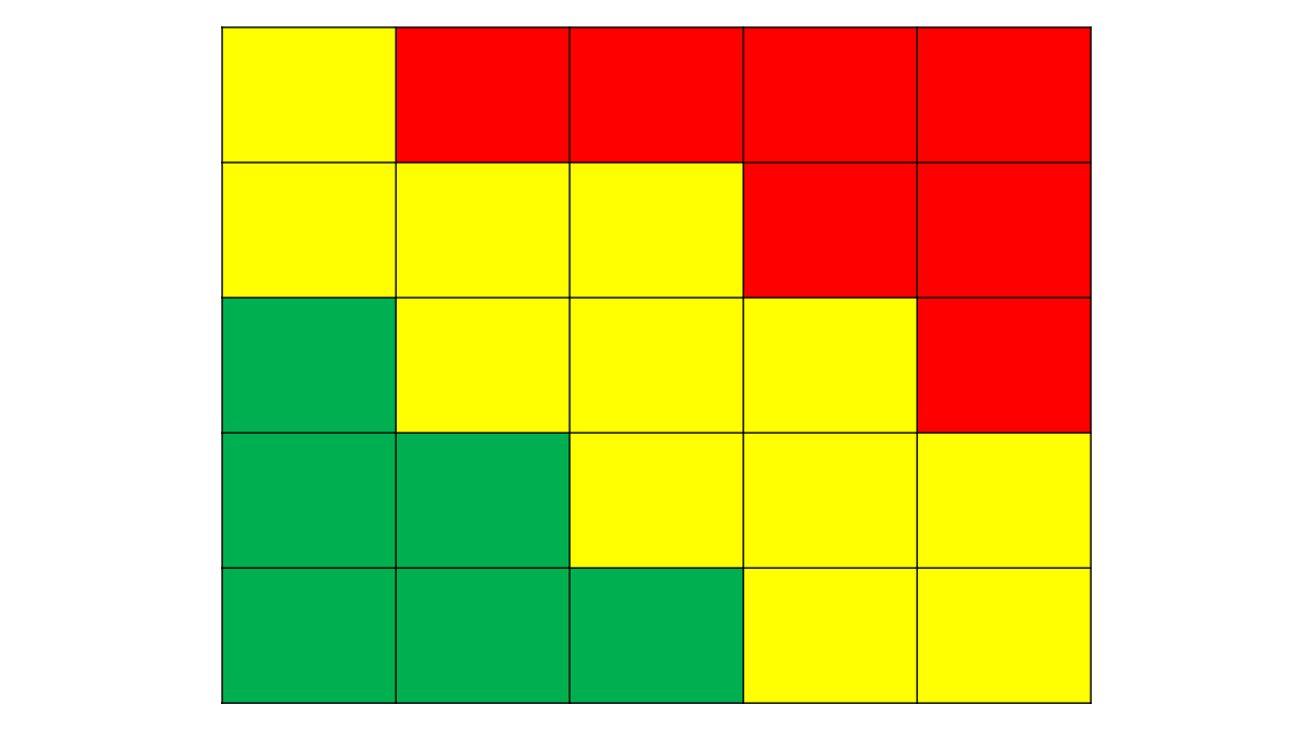
\includegraphics[width=1.0\textwidth]{Figures/example_figure1.JPG}
    \caption{Example figure 1.}
    \label{fig:example_figure1}
    \end{figure}
    
    %Bare for å generere noe tekst for å se hvordan det ser ut:
    \lipsum[1]
    
    \subsection{Name of subsection 1}
    %Bare for å generere noe tekst for å se hvordan det ser ut:
    \lipsum[1]
    
    \subsection{Name of subsection 2}
    %Bare for å generere noe tekst for å se hvordan det ser ut:
    \lipsum[1]
    
    \section{Name of section 2}
    
    %Bare for å generere noe tekst for å se hvordan det ser ut:
    \lipsum[1]
    
    \section{Name of section 3}
    %Bare for å generere noe tekst for å se hvordan det ser ut:
    \lipsum[1]
    
    \subsection{Name of subsection 1}
    %Bare for å generere noe tekst for å se hvordan det ser ut:
    \lipsum[1]
    
    \subsection{Name of subsection 2}
    %Bare for å generere noe tekst for å se hvordan det ser ut:
    \lipsum[1]
    
%%%%%%%%%%%%%%%%%%%%%%%%%%%%%%%%%%%%%%%%%%%%%%%%%%%%%%%%%%%%%%%
\biblio
\cleardoublepage
\end{document}